%!TEX root = ../template.tex

\chapter{Validation and Experimental Evaluation}
\label{cha:validation_experimental_Evaluation}

This chapter presents, analyses and discusses the work performed to obtain relevant evaluation criteria measured from the complete system deployed on a cloud environment, in order to validate the implemented prototype.

Section \ref{sec:testbench_environment} details how the system is deployed, explains the different configurations that that system adopts in order to present relevant data to compare.

In section \ref{sec:revelant_evaluation_criteria} explains which metrics will be evaluated for each different testbench scenario. Sections \ref{sec:performance_evaluation_redis_benchmark_tool} through \ref{sec:complementary_measurements} presents the actual metrics taken from the performance and load testing tools and compares the different system configurations with secure and vulnerable storage instances.

The last section, section \ref{sec:summary_and_findings} contains a summary of all the finding and some considerations that can be taken from the presented metrics.

\section{Testbench Environments}
\label{sec:testbench_environment}

The prototype was evaluated in multiple different system configurations to achieve a complete coverage of all the proposed solutions and all the relevant metrics. 

The first test is a representative test of the overhead introduced not only of additional security features like \gls{TLS} and authentication but also the \gls{SGX} hardware isolation. It will run the \textit{redis-benchmark} tool both externally to the server and internally directly against a single standalone Redis instance bypassing the proxy server. Secondly, and more real-life tests, test are run against the proxy exposed \gls{API} and a single standalone Redis instance composes the storage server. Then, the same tests were run in the same environment but with a cluster of Redis instances composing the backend storage. The fourth testbench measures the performance of homomorphic operations on a standalone Redis instance running on unprotected memory, and finally, it is presented the metrics for the two different attestation operations on Redis instances deployed on protected memory and isolated through \gls{SGX}.

All tests performed on the secure prototype are measured several times, averaged and compared with a standard Redis deployment so the overhead of extra security can be evaluated and analysed. 

\section{Relevant Evaluation Criteria}
\label{sec:revelant_evaluation_criteria}

The tests measure several different relevant metrics that can be compared with each other: 

\begin{itemize}
  \item \textbf{Latency} - Measured in milliseconds (ms) and evaluate the round trip response times between the client and the server.
  \item \textbf{Throughput} - Measured in operations per seconds (ops/s) indicates the number of operations the client performed in one second.
  \item \textbf{Startup Times} - Measured in seconds (s) is particularly important to analyse the \gls{SGX} attestation that happens at startup
  \item \textbf{Memory Consumption} - Extracted in megabytes (MB) or a percentage, and measured alongside the tests.
  \item \textbf{\gls{CPU} Consumption} - Extracted in megabytes in a percentage, and also measured alongside the tests.
\end{itemize}

\section{Performance Evaluation for Redis-Benchmark tool}
\label{sec:performance_evaluation_redis_benchmark_tool}

The first testbench is performed directly against the Redis server bypassing the proxy. This test was performed with the \textbf{redis-benchmark} \footnote{Since Redis TLS is fairly new, the latest official redis-benchmark realest does not support TLS test. The redis benchmark used comes from the Redis unstable branch (commit a0576bd), but after some analyses it appears to be a final version of the tool. All benchmarks tests used the same version} tool and evaluates the latency and throughput of a basic set of operations - \textit{ping}, \textit{set}, and \textit{get}. It compares three different deployed Redis configurations, where the first one is completely default and open, the second one implements the built-in security features of Redis such as \gls{TLS} and authentication and the third one, not only using the built-in features but also running isolated inside an \gls{SGX} enclave.

Figure \ref{fig:redis_benchmark_external_metrics} presents the latency and throughput results over one hundred thousand requests with 50 multiple concurrent clients and a 3 byte payload when running the benchmark tool on a Macbook Pro 2018 2,3 GHz Quad-Core Intel Core i5 and internet connection averaging the 500Mb/s download and 100Mb/s upload.

\begin{figure}[htbp]
  \centering
  \subcaptionbox{Redis Latency Result\label{fig:redis_latency_external}}%
    {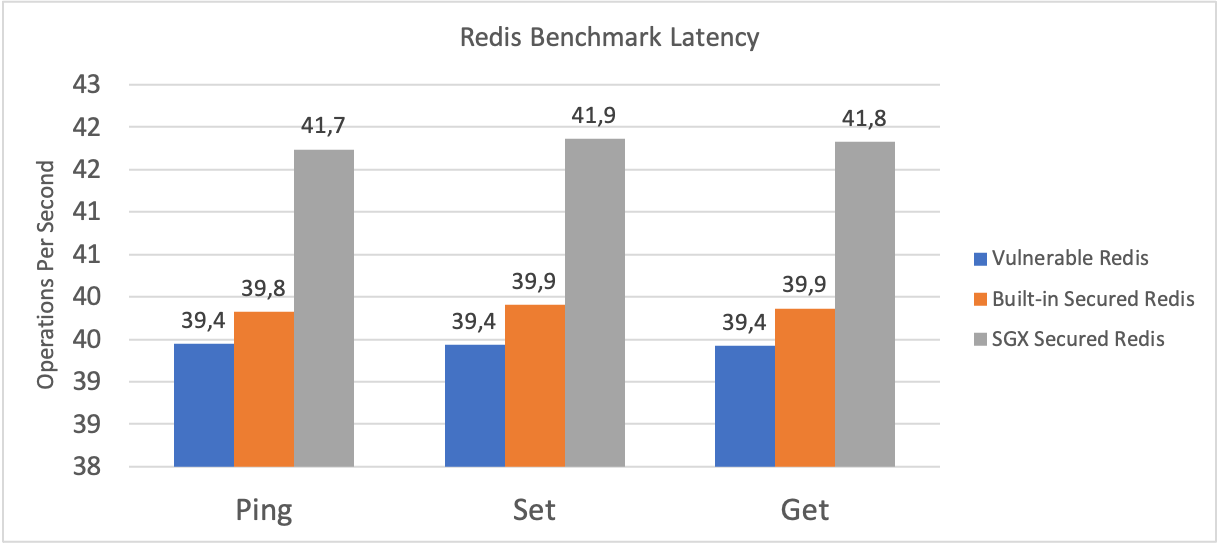
\includegraphics[width=0.5\linewidth]{redis_latency_external}}%
    %\hspace{1em}
  \subcaptionbox{Redis Throughput Result\label{fig:redis_throughput_external_2}}%
    {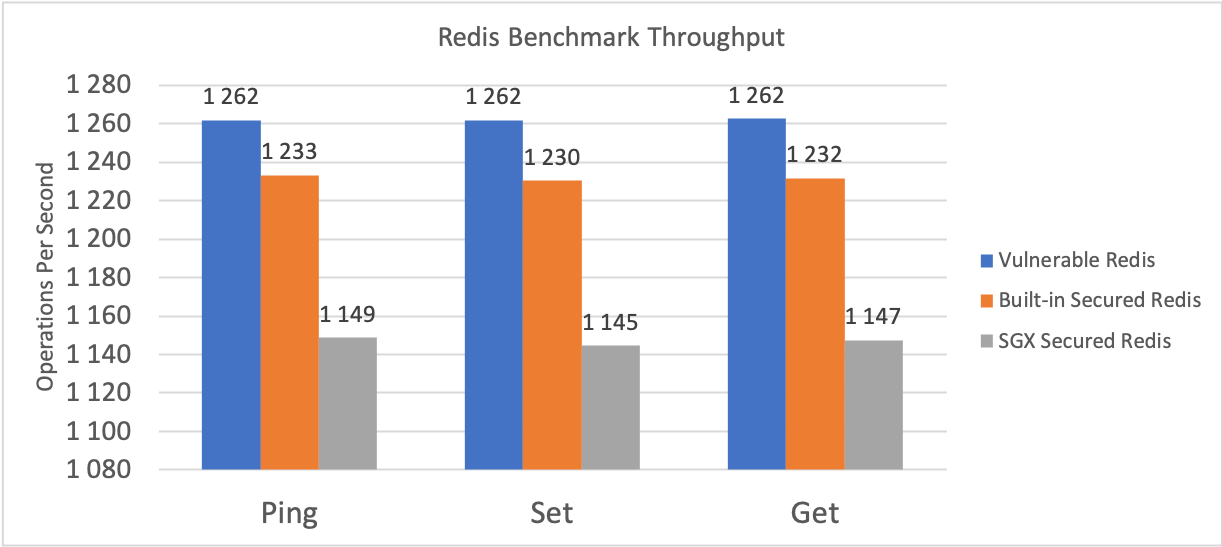
\includegraphics[width=0.5\linewidth]{redis_throughput_external_2}}%
  \caption{Redis Benchmark External Client Metrics}
  \label{fig:redis_benchmark_external_metrics}
\end{figure}

The results show a performance drop for each additional security layers added to the instance deployment. The \gls{SGX} deployed instance showed the biggest overhead on performance, around 8\%-10\%, both latency and throughput, however, due to the added security, this is an expected result.

Figure \ref{fig:redis_benchmark_internal_metrics} shows the results of the same tests but instead of running the benchmark tool on a separate machine, it runs it on the same host where the server is deployed, therefore eliminating the network overhead.

\begin{figure}[htbp]
  \centering
  \subcaptionbox{Redis Latency Internal\label{fig:redis_latency_internal}}%
    {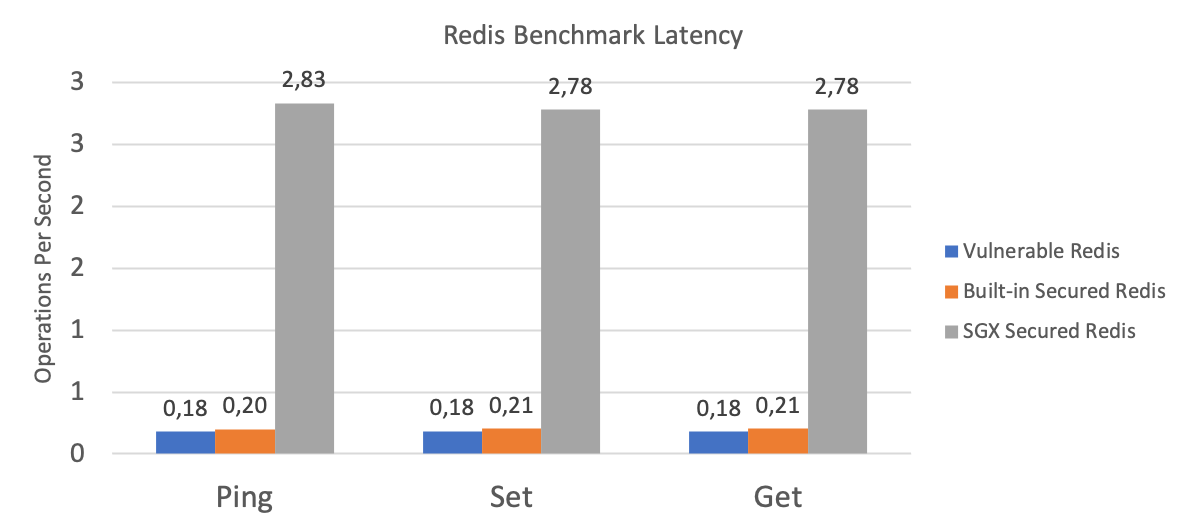
\includegraphics[width=0.5\linewidth]{redis_latency_internal}}%
    %\hspace{1em}
  \subcaptionbox{Redis Throughput Internal\label{fig:redis_throughput_internal}}%
    {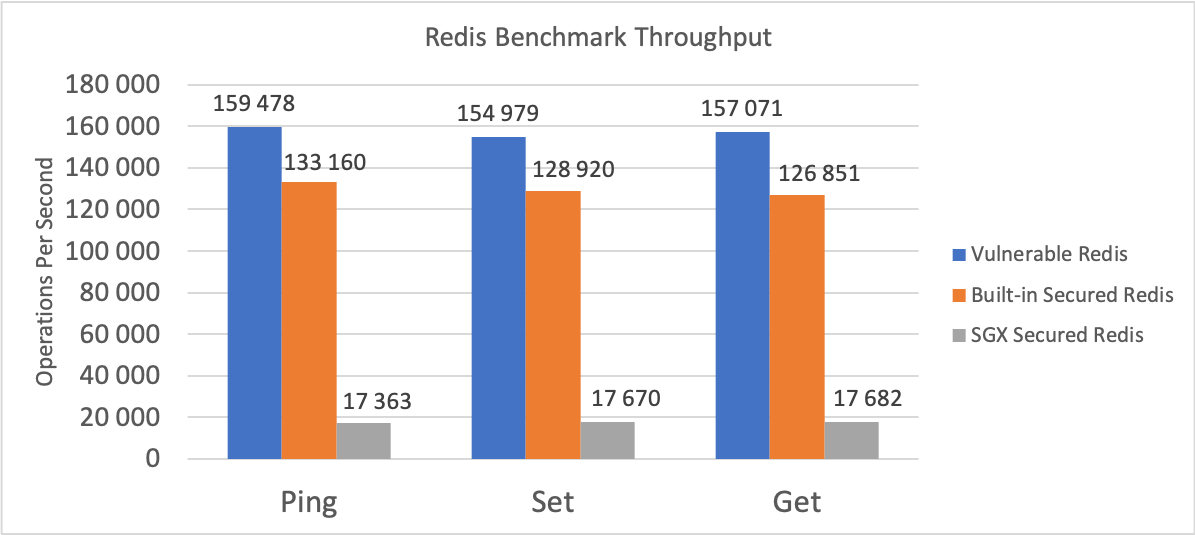
\includegraphics[width=0.5\linewidth]{redis_throughput_internal}}%
  \caption{Redis Benchmark Internal Client Metrics}
  \label{fig:redis_benchmark_internal_metrics}
\end{figure}

The results corroborate the initial tests but the differences between security levels are much more visible. The main objective of this comparison is to point out that the network jitter and latency overhead will affect the performance results going forward to the next tests.

\section{Performance Evaluation for Standalone Redis}
\label{sec:performance_evaluation_standalone_redis}

This testbench configuration tests a standalone architecture with a single proxy instance and a single Redis instance. Both the proxy and the Redis components will be tested in different deployment configurations, running inside and outside \gls{SGX} enclaves. When Redis is running outside the isolated environment, it will run both in a vulnerable configuration, without any security properties and in its encrypted format, where the proxy server enabled encrypted values.

The tests will run one single thread, making as many \textit{gets} and \textit{sets} requests as possible during 10 minutes with a 20 byte key and a 100 byte value. Figure \ref{fig:standalone_throughput_results} presents the throughput obtained from the tests for the different configurations.

\begin{figure}[htbp]
  \centering
  \subcaptionbox{Get throughput\label{fig:standalone_get_throughput}}%
    {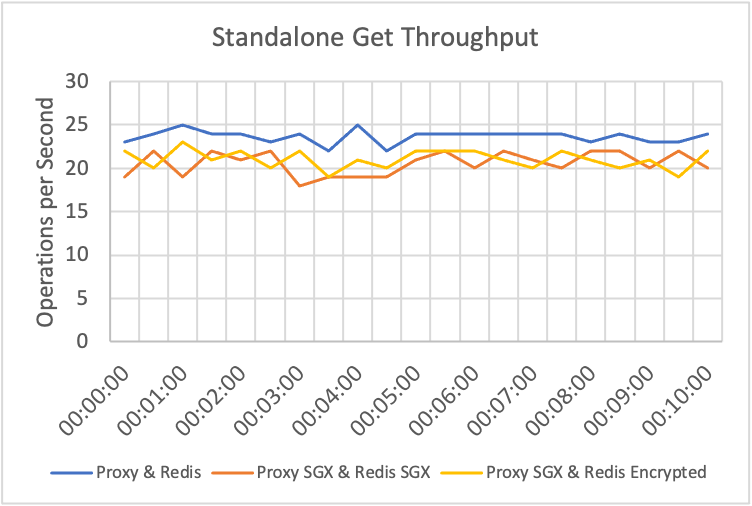
\includegraphics[width=0.5\linewidth]{standalone_get_throughput}}%
    %\hspace{1em}
  \subcaptionbox{Set throughput\label{fig:standalone_set_throughput}}%
    {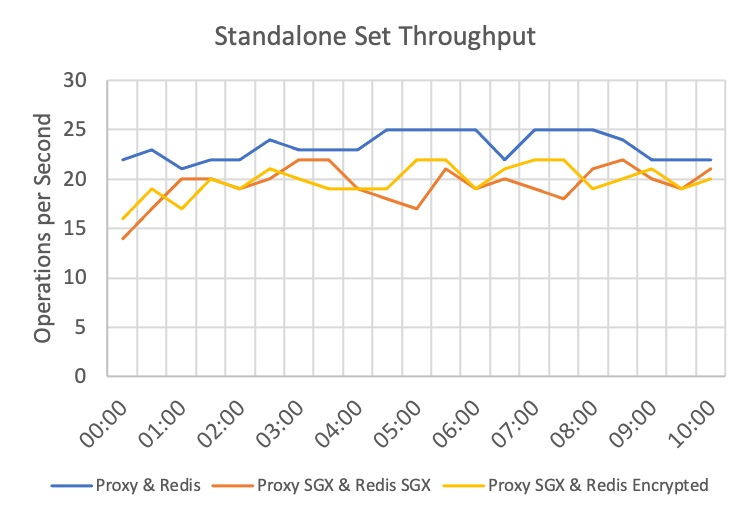
\includegraphics[width=0.5\linewidth]{standalone_set_throughput}}%
  \caption{Standalone Throughput Results}
  \label{fig:standalone_throughput_results}
\end{figure}

The throughputs measured from the different system configurations show a higher count of operations per second on the normal and vulnerable Proxy \& Redis configuration. When running the components on an \gls{SGX} enclave, performance takes a 20\%-25\% hit. Keeping the proxy running inside enclaves, but extracting the Redis to unprotected memory sees 18\%-22\% loss in performance. Even though the storage service is running faster outside enclaves, the proxy needs to perform extra work in order to maintain data privacy and integrity.
 
The latency results summarised on table \ref{tab:proxy_redis_standalone_latency_results} support the throughput measurements.

\begin{table}[ht]
	\caption{Proxy Redis Standalone Results}
	\label{tab:proxy_redis_standalone_latency_results}
\centering
\begin{tabular}{lccccc}
	\toprule
	\multicolumn{1}{c}{\textbf{Test}} & \pmb{\#}\textbf{Request} & \textbf{Avg Latency} & \pmb{\ensuremath{\sigma}} & \textbf{95}\pmb{\%} & \textbf{DB Size} \\
	\midrule
		Proxy \& Redis & 14038 & 42ms & 15ms & 42ms & 2,03MB 	\\
		Proxy SGX \& Redis SGX & 12013 & 49,67ms & 19,66ms & 58ms & 2,00MB \\
		Proxy SGX \& Redis Encrypted & 12773 & 48,67ms & 20,12ms & 55ms & 6,49MB \\
	\bottomrule
\end{tabular}
\end{table}

\section{Performance Evaluation for Cluster Redis}
\label{sec:performance_evaluation_cluster_redis}

%TODO: Write

Clustering on Redis is distributed out of the box on the latest Redis versions. It combines the Master-Slave model and an event bus to provide replication and sharding and coordination between the nodes. This test uses a configuration with one proxy server, and six Redis nodes, with three masters and three slaves. The tests run were the same of the standalone system configuration presented on section \ref{sec:performance_evaluation_standalone_redis} to maintain consistency between tests, and it runs a single thread, making as many requests as possible during 10 minutes, using random 20 byte keys with a 100 byte random value. Figure \ref{fig:cluster_throughput_results} shows the throughput results on the sets and get operations.

\begin{figure}[htbp]
  \centering
  \subcaptionbox{Get throughput\label{fig:cluster_get_throughput}}%
    {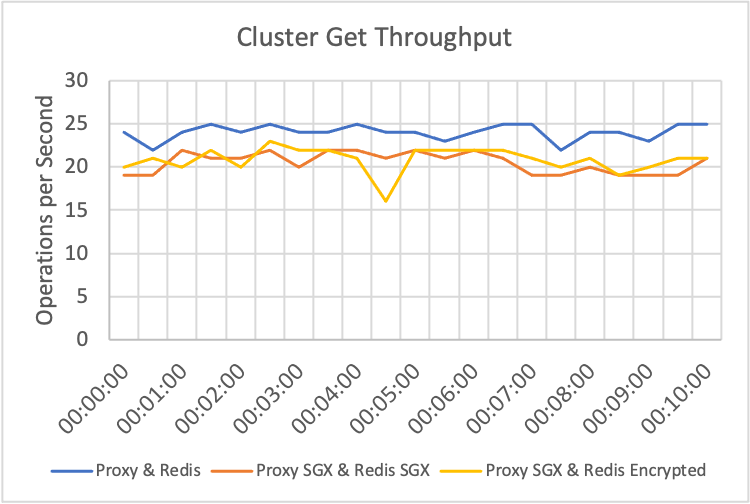
\includegraphics[width=0.5\linewidth]{cluster_get_throughput}}%
    %\hspace{1em}
  \subcaptionbox{Set throughput\label{fig:cluster_set_throughput}}%
    {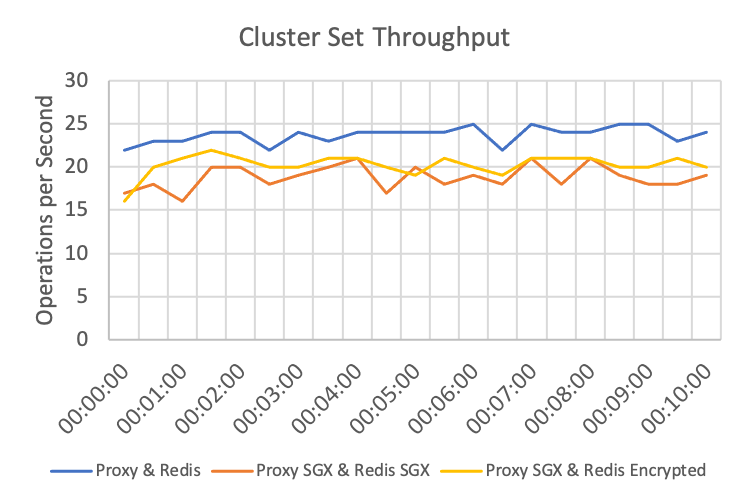
\includegraphics[width=0.5\linewidth]{cluster_set_throughput}}%
  \caption{Cluster Throughput Results}
  \label{fig:cluster_throughput_results}
\end{figure}

Again, as expected, the vulnerable Redis configuration is the fastest since it doesn't need to maintain any security or privacy properties. Running the Proxy and Redis server on an isolated environment incurs in a performance penalty. However, running the Redis in unprotected memory but on an encrypted format seems to have a bit of an edge in performance over the \gls{SGX} isolated server.

\begin{table}[ht]
	\caption{Proxy Redis Cluster Results}
	\label{tab:proxy_redis_cluster_latency_results}
\centering
\begin{tabular}{lccccc}
	\toprule
	\multicolumn{1}{c}{\textbf{Test}} & \pmb{\#}\textbf{Request} & \textbf{Avg Latency} & \pmb{\ensuremath{\sigma}} & \textbf{95}\pmb{\%} \\
	\midrule
		Proxy \& Redis & 14219 & 41ms & 13ms & 41ms  				\\
		Proxy SGX \& Redis SGX & 12229 & 49ms & 21ms & 53ms  		\\
		Proxy SGX \& Redis Encrypted & 13131 & 46ms & 16ms & 46ms 	\\
	\bottomrule
\end{tabular}
\end{table}

Table \ref{tab:proxy_redis_cluster_latency_results} shows the latency results of the same tests, and it shows a correlation with the tests and the evaluation made above.

By observing both throughputs and latencies of the standalone and the cluster configurations we can compared them and observe similarities. Both tests seem to have a similar result on all system configurations and that might be due to the consistency guarantee of the cluster. Although a Redis cluster does provide replication, automatically split data among multiple nodes and some availability during network partitions, it is not able to guarantee \textbf{strong consistency}. This means that under some specific conditions the Redis cluster can lose writes that were acknowledged to the user by the system. This happens because Redis uses asynchronous replication, where it responds to the client before replicating the results to the replica instances. This configuration explains the similarity in performance since the proxy will only communicate with one instance at a time and that instance will respond before replicate the given command, just like a standalone node.

\section{Performance Evaluation for Homomorphic Operations}
\label{sec:performance_evaluation_homomorphic_operations}

The implementation of homomorphic encryption is a way to speed up performance by performing arithmetic operations over encrypted data. This test runs a proxy server inside an \gls{SGX} enclave and a single Redis instance running on unprotected memory. To maintain data privacy and integrity on an unprotected Redis instance, the proxy enables encryption and only stores encrypted data on Redis. This test compares latency and throughputs of the \textit{Sum} and \textit{Search} operations of the system. There are three configurations to test, one where the proxy does not encrypted data (the plain Redis), a second where the proxy enables encryption with homomorphic ciphers, and the last one, where proxy encrypts data with standard \textit{AES} encryption. With homomorphic encryption, the operations are performed over the encrypted value, meaning that, unlike standard encryption, it does not need to decrypt the current value for the \textit{SUM} operation to succeed.

The \textit{Sum} tests were run over a dataset of 5000 key-pairs and over 5 minutes making as many requests as possible and the \textit{Search} test run over a dataset with 1 list with 1000 values with about 140 bytes per line. The tests were run multiple times with multiple payload sizes and the average throughputs and latencies are presented in figure \ref{fig:homomorphic_encryption_throughput_results} and table \ref{tab:sum_latency_results}.

\begin{figure}[htbp]
  \centering
  \subcaptionbox{\textit{Sum} Throughput\label{fig:sum_throughput_results}}%
    {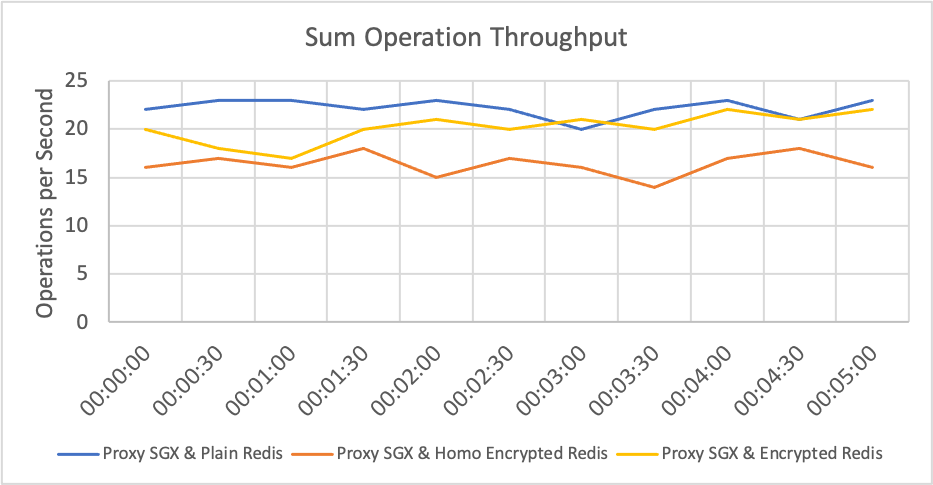
\includegraphics[width=0.5\linewidth]{sum_operation_throughput}}%
    %\hspace{1em}
  \subcaptionbox{\textit{Search} Throughput\label{fig:search_throughput_results}}%
    {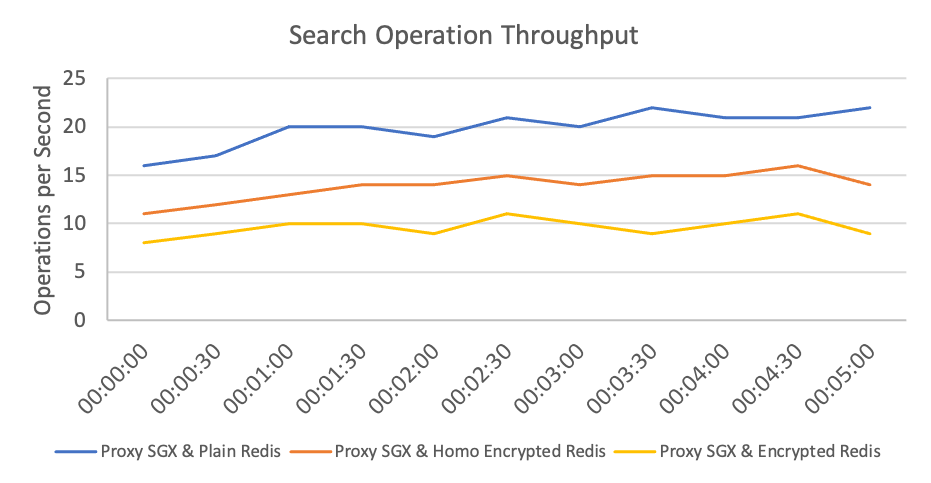
\includegraphics[width=0.5\linewidth]{search_operation_throughput}}%
  \caption{Homomorphic Encryption Throughput Results}
  \label{fig:homomorphic_encryption_throughput_results}
\end{figure}

\begin{table}[ht]
	\caption{\textit{Sum} Latency Results}
	\label{tab:sum_latency_results}
\centering
\begin{tabular}{lccccc}
	\toprule
	\multicolumn{1}{c}{\textbf{Test}} & \pmb{\#}\textbf{Request} & \textbf{Avg Latency} & \pmb{\ensuremath{\sigma}} & \textbf{99}\pmb{\%} & \textbf{DB Size} \\
	\midrule
		Sum - Plain Redis & 6512 & 46ms & 17ms & 48ms & 1.13MB  					\\
		Sum - Homo Encrypted Redis & 4853 & 62ms & 23ms & 69ms & 10.578MB  		\\
		Sum - Standard Encrypted Redis & 6001 & 52ms & 19ms & 54ms & 3.85MB  	\\
		Search - Plain Redis & 5718 & 52ms & 20ms & 68ms & 0.21MB				\\
		Search - Homo Encrypted Redis & 4238	 & 70ms & 25ms & 117ms & 0.49MB		\\
		Search - Standard Encrypted Redis & 3016	 & 99ms & 30ms & 150ms & 0.27MB	\\
	\bottomrule
\end{tabular}
\end{table}

As expected, a non encrypted Redis is the fastest configuration, however, the results on the encrypted configurations of the \textit{Sum} operation were not as anticipated. We were not able to achieve better performance by performing \textit{Sum} operations over encrypted data. This result maybe due to the size of the \textit{Sum} operation values, since we are working within the range of integers, standard \gls{AES} encryption is very fast. As we can see on the \textit{Search} operations, since values are strings, they are much bigger than a single integer and the encryption and decryption cycles are much more costly.

On the other hand, homomorphic encryption can enable operations that are not possible with the standard encryption like maintaining encrypted data in order and searching through finding values between certain boundaries. Other very important feature that is enabled by homomorphic encryption is that the plain text value is never present in memory, since the operations do not need to decrypt the value in order to proceeded.

\section{Evaluation of the Attestation Protocol}
\label{sec:evaluation_attestation_protocol}

The two different attestation types are evaluated in two different ways. Since hardware \gls{SGX} attestation is performed at container startup, it is evaluated by measuring the component deployment time and comparing it to a non-attested container.

Table \ref{tab:sgx_attestation_results} shows the comparison between startup times of the Redis instance and Proxy instance, both using, and not using \gls{SGX} hardware attestation.

%TODO: Add non enclave startup, enclave but no attestation, enclave and attestation and extrapolate attestation times

\begin{table}[ht]
	\caption{SGX Hardware Attestation Results}
	\label{tab:sgx_attestation_results}
\centering
\begin{tabular}{lccccc}
	\toprule
	\multicolumn{1}{c}{\textbf{Component}} & \textbf{No Attestation} & \textbf{SGX Attestation} & \textbf{Time Loss} \\
	\midrule
		Redis Instance & 0,009s & 1,604s & 1,594s 	\\
		Proxy Instance & 3,108s & 69,146s & 66,038s 	\\
	\bottomrule
\end{tabular}
\end{table}

On the other attestation type, the proxy will contact the Redis instance and get a signed quote of important aspects of the system such as the binary and configuration file, \gls{OS} kernel information and \gls{CPU} core count and processor type. It also attests itself and returns the quotes to the client. This processes was also measured by requesting as much attestation quotes in 10 minutes and collected throughputs and latency values described on table \ref{tab:custom_attestation_results}.

\begin{table}[ht]
	\caption{Custom Attestation Results}
	\label{tab:custom_attestation_results}
\centering
\begin{tabular}{lccccc}
	\toprule
	\multicolumn{1}{c}{\textbf{Run Number}} & \pmb{\#}\textbf{Request} & \textbf{Avg Latency} & \pmb{\ensuremath{\sigma}} & \textbf{99}\pmb{\%} & \textbf{Req/s} \\
	\midrule
		1st Run & 1491 & 402ms & 188	ms & 549ms & 2,481 ops/s \\
		2nd Run & 1494 & 401ms & 179	ms & 550ms & 2,483 ops/s \\
		3rd Run & 1494 & 401ms & 164ms & 546ms & 2,486 ops/s \\
	\bottomrule
\end{tabular}
\end{table}

\section{Complementary Measurements}
\label{sec:complementary_measurements}

Memory, CPU, etc instrumentation, workload

Exhausting SGX memory

\section{ Summary and Findings}
\label{sec:summary_and_findings}

% \section{Performance evaluation for Testbench 1}
% \label{sec:performance_evaluation_testbench_1}

% \subsection{Latency}
% \label{ssec:testbench_1_latency}

% \subsection{Throughput}
% \label{ssec:testbench_1_throughput}

% \section{Performance evaluation for Testbench 2}
% \label{sec:performance_evaluation_testbench_2}

% \subsection{Latency}
% \label{ssec:testbench_2_latency}

% \subsection{Throughput}
% \label{ssec:testbench_2_throughput}

% \section{Evaluation of the Attestation Protocol}
% \label{sec:evaluation_attestation_protocol}

% Get startup times with and without CAS, get stack attestation times...

% \section{Complementary Measurements}
% \label{sec:complementary_measurements}

% Memory, CPU, etc instrumentation, workload

% \section{ Summary and Findings}
% \label{sec:summary_and_findings}
